%% Language Resources and Evaluation version of the paper, built by paper/make_lre.py from paper/main.tex.
%% Template: Springer Nature LaTeX template (sn-jnl, Version 3.1, December 2024), APA reference style (author-year).
%% Submit this one .tex file with references.bib (and main.bbl), sn-jnl.cls, sn-apacite.bst and the figure files.
\documentclass[pdflatex,sn-apa]{sn-jnl}

\usepackage{graphicx}%
\usepackage{multirow}%
\usepackage{amsmath,amssymb}%
\usepackage[title]{appendix}%
\usepackage{xcolor}%
\usepackage{booktabs}%
\usepackage{array}%
\usepackage{tabularx}%

\newcommand{\BHS}{\textsc{bhs}}

\raggedbottom

\begin{document}

\title[Genre Routing for Bangla Hallucination Judges]{Does Genre Routing Help LLM Hallucination Judges? Evidence from Bangla}

\author*[1]{\fnm{Mahdi Hasan} \sur{Qurishi}}\email{mahdiqureshi9@gmail.com}

\author[1]{\fnm{Umme Zoayria} \sur{Abedin}}

\author[1]{\fnm{Md Saminul} \sur{Amin}}

\affil*[1]{\orgdiv{Department of Computer Science and Engineering}, \orgname{Shahjalal University of Science and
Technology}, \orgaddress{\city{Sylhet}, \postcode{3114}, \country{Bangladesh}}}

\abstract{Large language models (LLMs) are widely used as judges that decide whether an answer is hallucinated, and a natural idea is routing each item to the judge that is strongest for its topic. We release \textbf{GenreHalluEval v2.0}, a Bangla benchmark for hallucination judges with 1,200 questions in 12 balanced genres, 6,000 gold and hallucinated answers, a fixed learn/test split, labels double-checked on a blind 20\% sample (Cohen's $\kappa$ 0.99) and the raw outputs of five open-weight judges, together with an audited BenHalluEval-QA set (920 questions) and the team-written GenreHalluEval v1.1 (250 questions). On these sets we compare three genre routes with the single best judge, with and without the passage: the best guesser's genre (E), each LLM's own genre (F) and the better of the two (R). In five tests, one of them preregistered, no route is clearly better than the single best judge, even before correction for multiple tests. Own-genre routing is clearly worse in four of the eight study-and-condition pairs, because a cell-size rule hands whole genres to weak judges. We turn these findings into a noise- and cost-aware protocol for judge evaluation: measure the judges' own run-to-run flip rate at temperature 0 (0.2--0.4\% of verdicts here), count the answers a route actually changes, and set the gain against its cost. Under this protocol, every apparent gain (two to six answers) lies within the noise floor, while costing 1.2 to 1.9 times the calls and 2.7 to 6.6 times the prompt tokens of the single best judge.}

\keywords{Bangla, Hallucination detection, LLM-as-a-judge, Benchmark dataset, Judge routing, Inference noise}

\maketitle

%==================================================================================================================
\section{Introduction}
%==================================================================================================================

LLMs are increasingly used to judge the output of other LLMs, including whether an answer is hallucinated, that is,
not supported by a source or not true \citep{zheng2023judging}. Benchmarks of such judges show that the best judge
changes from task to task \citep{benhallueval}. This suggests a simple improvement: if judges differ by topic, send
each item to the judge that is strongest for that topic. Routing among judges by slice is an active research direction
\citep{judgepanels2026,juryondemand2025}, and routing answering models by domain is well studied
\citep{shnitzer2023routing,inferencedynamics2025,archrouter2025}.

Two questions decide whether topic routing is useful in practice. First, are the topic strengths of judges stable, so
that a route learned on one set of items still holds on new items? Second, does a stable gain pay for the extra cost
of routing, which must first find the topic and may then call a different, often slower, judge? We study both
questions for Bangla, a widely spoken language with few evaluation resources, using \emph{genre} (the topic area of a
question, such as history, science or religion) as the routing key.

Answering these questions needs data that do not yet exist for Bangla: a benchmark whose genres are balanced
and fine enough that every genre has enough questions to learn a route on, with a fixed split, reliable labels and the
raw outputs of several judges. We build such a benchmark, GenreHalluEval v2.0, and two smaller sets, and release them
with every prompt, run and script.

We start from the question-answering (QA) task of BenHalluEval \citep{benhallueval}, a Bangla hallucination-detection
benchmark. A judge reads a question and an answer, with or without a supporting passage, and replies whether the
answer is hallucinated. We audited the QA seeds, wrote new hallucinated answers (the original ones are not in the
public release), labelled every question with a genre and ran twelve open-weight judges. We then preregistered a test
of genre routing on a new, team-written test set. The registered test found no gain. Because a negative result can
have many causes, we ran four follow-up tests that removed the most likely ones: a change of dataset between learning
and testing, coarse merged genres, unbalanced genres and small cells. Along the way we found that the
differences routing produces are of the same size as the judges' own run-to-run noise at temperature 0, which most
judge comparisons ignore. We therefore frame the result not only as ``routing does not help'' but as a guardrail: a
protocol that tells practitioners when an apparent gain of one judge set-up over another is real and worth its cost.

\paragraph{Contributions.}
\begin{itemize}
  \item \textbf{GenreHalluEval v2.0, a reusable Bangla benchmark for hallucination judges.} 1,200 questions in 12
  balanced genres (including Bangla grammar), 6,000 answers, a fixed learn/test split, a blind 20\% double check
  ($\kappa$ 0.990 for answers, 0.991 for genres), per-genre baselines and the raw outputs of five judges, ready for
  genre-level judge evaluation and routing research (Section~\ref{sec:v2}). We also release an audited
  BenHalluEval-QA set (920 questions, human-verified genre labels) and GenreHalluEval v1.1 (250 team-written
  questions, double-labelled) (Section~\ref{sec:data}).
  \item \textbf{A noise- and cost-aware protocol for evaluating judge routing.} Five checks: the judges' run-to-run
  noise floor, a paired bootstrap over questions, the answers a route actually changes, its cost per fixed answer,
  and a coverage check for own-genre routes (Section~\ref{sec:protocol}).
  \item \textbf{A consistent negative result.} In five tests (one preregistered, four exploratory), no genre route
  is clearly better than the single best judge, even before correction (Section~\ref{sec:results}). The result holds
  with fine, balanced genres.
  \item \textbf{Own-genre routing and its failure mode.} A route in which each LLM names the genre and is scored
  inside the genre it named itself (F) is clearly worse than the single best judge in four of the eight
  study-and-condition pairs; a minimum cell size leaves the strong judges without cells in some genres, so whole genres
  go to weak judges (Section~\ref{sec:whyf}).
\end{itemize}

%==================================================================================================================
\section{Related work}
%==================================================================================================================

\paragraph{LLMs as judges.} LLM judges are now a standard way to evaluate open-ended output \citep{zheng2023judging}.
Their verdicts depend on the judge: swapping or upgrading a judge changes measured results
\citep{judgechanges2026}. Without a reference, judges agree with experts mainly on questions they can answer
themselves \citep{nofreelabels2025}, and when a reference is given, judges can still over-rely on their own knowledge
when the two conflict \citep{judgingreference2026}. We therefore report every result separately with the passage and
without it.

\paragraph{Routing among judges.} The closest work routes among the members of a judge panel by declared slices: from
a small labelled audit set it finds judges that help only on some slices and calls them only there
\citep{judgepanels2026}. Other work selects the most reliable judges per item with learned reliability predictors
\citep{juryondemand2025}, or routes each query to a reasoning or a non-reasoning judge under a budget
\citep{racer2026}. We do not propose a new routing algorithm. We test whether genre-based routes for hallucination
judges hold on new data, in Bangla, and we add own-genre routing.

\paragraph{Routing answering models.} Routing among answering models by domain or category is well studied:
learning from benchmark data which model to use on new tasks \citep{shnitzer2023routing}, routing by capability and
domain profiles \citep{inferencedynamics2025} and by user-defined categories \citep{archrouter2025}. Self-routing lets
each answering model judge its own competence \citep{disrouter2025}. Own-genre routing is related but different: we
never ask a model about its competence; we use its \emph{measured} score inside the genre it names, and we route judges,
not answering models.

\paragraph{Bangla hallucination evaluation.} BenHalluEval \citep{benhallueval} is a multi-task Bangla
hallucination-detection benchmark with nine judges and the BenHalluScore (\BHS{}) metric; its QA seeds come from the
Bengali part of TyDi QA \citep{clark2020tydi}. We use only its QA task and re-run every judge ourselves.

%==================================================================================================================
\section{Data}\label{sec:data}
%==================================================================================================================

Every set has the same structure. A \emph{question} has a passage, a question text and a gold answer. Each question
has five \emph{answers}: the gold and four hallucinated answers, one of each type used by BenHalluEval QA: a wrong fact
of the same kind (F, factualness), a misread question, usually another span of the passage (C, comprehension), the
gold plus a false detail (S, specificity) and a wrong inference (I). The passage defines the truth. Every hallucinated
answer in this paper was written by an LLM (Claude, Anthropic) under a fixed writing guide (Appendix~\ref{app:ai});
none is an output of the judged models. Table~\ref{tab:data} summarises the sets.

\begin{table}[t]
\centering\small
\caption{The four evaluation sets. Every question has 1 gold and 4 hallucinated answers. Kappa values are Cohen's
$\kappa$ between two people labelling alone, except where marked.}\label{tab:data}
\begin{tabularx}{\textwidth}{@{}l r r X X@{}}
\toprule
Set & Questions & Genres & Source of questions and golds & Human checks \\
\midrule
BenHalluEval-QA v1.3 & 920 & 5 + Other & TyDi QA (Bengali) via BenHalluEval; audited & genre: all 997 questions verified; blind 200, $\kappa$ 0.770; answer labels: 200 answers, $\kappa$ 0.969 \\
GenreHalluEval v1.1 & 250 & 5 $\times$ 50 & written by the team & genre: 3 annotators, Fleiss' $\kappa$ 0.987; answer labels: all 1,250, $\kappa$ 0.990 \\
GenreHalluEval v2.0 & 1,200 & 12 $\times$ 100 & 230 from v1.1; 970 written by Claude from Bangla Wikipedia and a school grammar book & blind 20\% sample: genre $\kappa$ 0.991 (240 questions); answer labels $\kappa$ 0.990 (969 answers) \\
\bottomrule
\end{tabularx}
\end{table}

\subsection{BenHalluEval-QA v1.3 (learning set of the registered test)}

BenHalluEval QA takes 1,000 hard questions from the Bengali part of TyDi QA GoldP \citep{benhallueval,clark2020tydi}.
The 4,000 hallucinated answers of the original benchmark, generated with GPT-5.4, are not in the public release, so we
wrote new ones of the same four types. We audited every seed: 139 gold answers did not fit their question; 50
time-sensitive golds were checked against the web and 22 were updated; after a review by the first author and a
second check against the current state of the world, duplicates and unfixable seeds were dropped. Version 1.3 has 920
questions and 4,600 answers.

\paragraph{Genres.} We froze a guide with five genres and Other (History, Politics \& Education; Arts, Culture \&
Sports; Science \& Technology; Geography \& Places; Religion) before seeing any judge result. An LLM drafted a genre
for each question; the first author verified all of them and changed 15 (1.5\%). We report these labels as
LLM-drafted and human-verified. On a blind set of 200 questions, the two human annotators agree at $\kappa=0.770$.

\paragraph{A shortcut.} Every gold is a span of the passage, while most hallucinated answers are not. The rule
``hallucinated if the answer is not an exact span of the passage'' scores \BHS{} 13.8 with the passage, without
reading the question. A judge must beat this to show that it reads the passage. The same property holds for the
original benchmark design.

\subsection{GenreHalluEval v1.1 (test set of the registered test)}

The team wrote 250 new questions with passages from Bangla sources (BanglaPedia, news sites and Wikipedia), 50 per
genre; the first author wrote the golds. Three annotators labelled the genres (Fleiss' $\kappa$ 0.987 \citep{fleiss1971}),
and 17 questions that overlapped with BenHalluEval were replaced. Each answer is judged in one condition: 175 questions
with the passage and 75 without it. Two annotators (the second and third authors) labelled all 1,250 answers alone
against the passage ($\kappa$ 0.990 \citep{cohen1960}); the four disagreements were settled before any score was
computed, and the agreed labels equal the design labels.

\subsection{GenreHalluEval v2.0: a balanced 12-genre benchmark}\label{sec:v2}

GenreHalluEval v2.0 is the main resource of this paper. We built it after the registered result, to remove two
possible causes of the null result: merged genres and small cells.

\paragraph{Composition.} Twelve single genres (History, Politics, Education, Arts, Culture, Sports, Science,
Technology, Geography, Places, Religion and Grammar) with exactly 100 questions each (Table~\ref{tab:v2comp}). It keeps
230 v1.1 questions whose genre fits one of the 12 and adds 970 questions written by Claude from current Bangla
Wikipedia revisions (title and revision id recorded) and, for 88 Grammar questions, from the national Bangla grammar
textbook for grades 9--10 \citep{nctb2021grammar}. The Grammar genre (sandhi, compounds, prefixes, word origins and
idioms) has no counterpart in the genre labels of BenHalluEval-QA. New questions were checked against BenHalluEval
for overlap.

\paragraph{Split.} A fixed split, stratified by genre and by origin (v1.1 or new): a learn half of 600 questions (50
per genre; every answer meant to be judged with and without the passage) and a test half of 600 (25 per genre with the
passage and 25 without). Routes or calibrations can be learned on the learn half and tested on the test half with
cells of 50 questions.

\paragraph{Quality.} Two annotators checked a blind, genre-stratified 20\% sample alone: 194 new questions (genre,
question quality and all 970 answers) and 46 kept v1.1 questions (genre). Answer labels agree at $\kappa=0.990$
between the annotators and 1.000 and 0.990 with the design labels; genres agree at $\kappa=0.991$; every sampled
question was judged clear and answerable. Both annotators marked exactly one correct answer per question, as in the
design, so agreement with the design is an upper bound. The other 80\% of the new questions are not human-checked.

\paragraph{Baselines and format.} Table~\ref{tab:v2base} gives the five judges' learn-half scores and the best judge's
test-half score per genre. The release has one CSV row per answer (item and question ids, genre, condition, passage,
question, answer, answer type, design label, source), the split, the lock and test plan of Study~3, checksums, and
every raw judge output with prompt hashes, tokens and latency.

\begin{table}[t]
\centering\small
\caption{GenreHalluEval v2.0: questions per genre, by origin. Every question has 1 gold and 4 hallucinated answers.}
\label{tab:v2comp}
\begin{tabular}{@{}lrrr@{\hspace{1.2cm}}lrrr@{}}
\toprule
Genre & v1.1 & New & Total & Genre & v1.1 & New & Total \\
\midrule
History & 13 & 87 & 100 & Science & 23 & 77 & 100 \\
Politics & 28 & 72 & 100 & Technology & 26 & 74 & 100 \\
Education & 4 & 96 & 100 & Geography & 33 & 67 & 100 \\
Arts & 33 & 67 & 100 & Places & 11 & 89 & 100 \\
Culture & 0 & 100 & 100 & Religion & 46 & 54 & 100 \\
Sports & 13 & 87 & 100 & Grammar & 0 & 100 & 100 \\
\midrule
\multicolumn{8}{@{}l}{All: 230 from v1.1, 970 new, 1,200 questions, 6,000 answers} \\
\bottomrule
\end{tabular}
\end{table}

\begin{table}[t]
\centering\small
\caption{GenreHalluEval v2.0 baselines (\BHS{}, lower is better). Left: each judge on the learn half (600 questions,
3,000 answers per condition). Right: the best judge, gemma4-31b, on the test half per genre (25 questions per genre
and condition).}\label{tab:v2base}
\begin{tabular}{@{}lrr@{\hspace{1cm}}lrr@{}}
\toprule
Judge (learn half) & With & Without & Genre (test half) & With & Without \\
\midrule
gemma4-31b & 0.33 & 21.96 & History & 1.00 & 14.00 \\
qwen3.5-27b & 0.88 & 23.10 & Politics & 1.00 & 29.00 \\
gpt-oss-20b & 4.15 & 32.44 & Education & 0.00 & 23.50 \\
deepseek-r1-14b & 20.98 & 29.79 & Arts & 0.00 & 28.50 \\
tigerllm-9b (Bangla prompts) & 36.12 & 40.92 & Culture & 0.00 & 15.00 \\
 & & & Sports & 0.00 & 22.50 \\
 & & & Science & 0.50 & 15.50 \\
 & & & Technology & 0.00 & 9.00 \\
 & & & Geography & 0.00 & 21.50 \\
 & & & Places & 0.00 & 29.00 \\
 & & & Religion & 1.00 & 19.00 \\
 & & & Grammar & 0.00 & 27.50 \\
\bottomrule
\end{tabular}
\end{table}

%==================================================================================================================
\section{Method}\label{sec:method}
%==================================================================================================================

\subsection{Judges, conditions and metric}

\paragraph{Conditions.} With the passage, a judge sees passage, question and answer (BenHalluEval's zero-shot judge
prompt, unchanged). Without the passage, it sees question and answer and must use its own knowledge. Every table,
choice and test is made separately for the two conditions.

\paragraph{Judges.} We ran twelve open-weight models on BenHalluEval-QA through Ollama\footnote{Ollama 0.40.6
(llama3.1-8b: 0.40.5), \url{https://ollama.com}.}: the nine models of BenHalluEval except GPT-4.1 mini, plus
gemma4-31b, qwen3.5-27b, gpt-oss-20b and an instruction-tuned TituLLM. Three Bangla-specific models (TituLLM-3B, its
instruction-tuned version and BanglaLLaMA-13B) produced no usable verdicts and were never routed to. The follow-up
studies use a pool of five: gemma4-31b, qwen3.5-27b, gpt-oss-20b, deepseek-r1-14b and tigerllm-9b. TigerLLM uses Bangla
prompts in those studies, because they improved its score without the passage on BenHalluEval (by 4.8 points);
every other model uses the same English instructions.

\paragraph{Settings.} Temperature 0, seed 2026, the context length set explicitly with a check that no prompt was cut,
strict parsing (``yes'' = hallucinated, ``no'' = not hallucinated, anything else = \emph{no answer}, counted as an
error), the thinking block of reasoning models removed before parsing and capped outputs counted as no answer. Every
call is logged with its prompt hash, tokens and latency. Runs used two NVIDIA T4 GPUs on Kaggle.

\paragraph{Metric.} BenHalluScore \citep{benhallueval}:
\begin{equation}
\BHS = \tfrac{1}{2}\left(\frac{\text{correct answers flagged}}{\text{correct answers}} +
\frac{\text{hallucinations missed}}{\text{hallucinated answers}}\right)\times 100 .
\end{equation}
Lower is better; 50 is chance or a judge that gives the same verdict to everything. Because only one answer in five is
correct, one false alarm costs four times as much as one miss.

\subsection{Routes}

Every route is learned on a \emph{learn} set and frozen in a lock file before the \emph{test} set is judged.
\begin{description}
  \item[A, single best judge:] the judge with the lowest overall \BHS{} on the learn set.
  \item[D, our genre:] the human genre label picks the best judge for that genre (a reference, not deployable).
  \item[E, guessed genre:] the LLM whose genre guesses agree most with the human labels on the learn set names the
  genre; the best judge for that genre judges.
  \item[F, own genre:] every LLM names the genre. Each LLM has a learn-set score inside the genre \emph{it} named
  (all learn questions it put in that genre, whatever the human label). The answer goes to the LLM with the best such
  score; if no LLM has a cell for the genre it named, to A.
  \item[R, best path:] the E path and the F paths compete, and the one with the lower learn-set score wins. Only the
  LLMs whose own-genre score can win are asked for the genre.
\end{description}
A cell (judge $\times$ genre) is used only if it has at least a minimum number of learn questions; otherwise the
route falls back to A. Ties go to the judge with the lower overall \BHS{}. Genre prompts never contain the answer, so
the genre cannot leak the label.

\subsection{Use of large language models}\label{sec:llmuse}

Claude (Anthropic; model claude-opus-5-5) was used in four roles, all checked by people as described in
Section~\ref{sec:data}: it wrote every hallucinated answer under a fixed writing guide (Appendix~\ref{app:ai}); it wrote
970 of the 1,200 GenreHalluEval v2.0 questions and their gold answers from cited sources, and transcribed the
grammar-book passages from page images; it drafted genre labels that people verified (BenHalluEval-QA) or checked on a
blind sample (v2.0); and it wrote the analysis code and helped draft the manuscript. Claude was never used as a judge or
as a genre guesser, so no judged model also wrote the answers it judged. The authors designed the study, ran all
experiments and take responsibility for the content.

\subsection{Statistics}

Every comparison is route minus A on the same test answers, with a 95\% range and a two-sided $p$ value from a paired
bootstrap that re-samples \emph{questions} (10,000 re-samples, seed 2026) \citep{efron1979}, because the five answers
of a question are not independent. Main tests are corrected with Holm's method \citep{holm1979}. We report cost
(calls, tokens, time) for every route.

\subsection{Five tests}

\begin{enumerate}
  \item \textbf{Study 1, registered, change of dataset.} Learn on BenHalluEval-QA v1.3 (the nine judges with usable
  verdicts, cells of 50+ questions), test on GenreHalluEval v1.1. Main tests: R vs A with and without the passage, Holm over 2. Registered
  on OSF before any test answer was judged (\url{https://osf.io/fmbs8}, embargoed).
  \item \textbf{Study 2a, split inside BenHalluEval.} The 920 questions are split in halves by genre (seed 2026); the
  lock rules are applied to one half and tested on the other, from the saved runs, plus 200 further random splits
  used in both directions.
  \item \textbf{Study 2b, split inside GenreHalluEval v1.1.} A learn half of 125 questions (every answer judged with
  and without the passage) and a test half of 125 (each answer in one condition); five judges; cells of 20+ questions,
  because a half has 25 questions per genre.
  \item \textbf{Study 3, GenreHalluEval v2.0.} A learn half of 600 questions (50 per genre; every answer judged with and
  without the passage) and a test half of 600 (25 + 25 per genre with and without the passage); five judges; cells of
  50+ questions; one notebook per route, so that each route's cost is measured on its own. Main tests: E, F and R vs A
  in both conditions, Holm over 6, fixed in a dated test-plan file after the learn run and before any test run.
\end{enumerate}
Studies 2a, 2b and 3 were designed after the result of Study 1. They are exploratory with respect to the registration
and are reported here in full, together with Study 1.

%==================================================================================================================
\section{Results}\label{sec:results}
%==================================================================================================================

\subsection{Judges on BenHalluEval-QA}

Table~\ref{tab:judges} shows the strongest judges. With the passage, gemma4-31b and qwen3.5-27b are far ahead
(\BHS{} 1.4 and 1.8) and well below the span shortcut (13.8); without it, every judge is much worse (31.9 and above).
This gap shapes everything that follows: with the passage, the best judge makes very few errors, so there is little
room for routing to help.

\begin{table}[t]
\centering\small
\caption{BenHalluEval-QA v1.3 (920 questions, 4,600 answers): \BHS{} of the judges with usable verdicts, with 95\%
ranges. Three Bangla-specific models gave no usable verdicts. The span rule needs the passage.}\label{tab:judges}
\begin{tabular}{@{}lrr@{}}
\toprule
Judge & With the passage & Without the passage \\
\midrule
gemma4-31b & \textbf{1.44} (0.95--1.94) & \textbf{31.92} (30.54--33.44) \\
qwen3.5-27b & 1.78 (1.33--2.23) & 32.85 (31.56--34.10) \\
gemma2-27b & 6.10 (5.45--6.79) & 38.18 (36.96--39.48) \\
gpt-oss-20b & 7.08 (6.15--8.03) & 39.76 (38.33--41.21) \\
qwen2.5-32b & 9.86 (9.04--10.75) & 37.43 (36.17--38.75) \\
deepseek-r1-14b & 22.76 (21.18--24.59) & 38.29 (36.67--39.92) \\
llama3.1-8b & 36.71 (35.41--38.03) & 45.98 (44.71--47.28) \\
tigerllm-9b & 38.82 (37.23--40.39) & 44.80 (43.74--45.90) \\
mistral-nemo-12b & 49.65 (47.98--51.26) & 50.75 (49.81--51.71) \\
\midrule
Rule: not a span of the passage & 13.82 & -- \\
\bottomrule
\end{tabular}
\end{table}

\subsection{No route beats the single best judge}

Table~\ref{tab:main} and Figure~\ref{fig:forest} give every route-versus-A comparison of the five tests.

\paragraph{Study 1 (registered).} Routes learned on BenHalluEval did not beat the single best judge (gemma4-31b) on
GenreHalluEval v1.1. R was slightly worse in both conditions: with the passage 0.86 vs 0.57 (+0.29, range $-0.07$ to
$+0.71$, Holm $p=0.37$), without it 22.83 vs 21.83 (+1.00, $-2.00$ to $+4.17$, Holm $p=0.55$). Both hypotheses of the
registration are not supported. With the passage, A made 5 errors in 875 answers; R made 9.

\paragraph{Study 2a (split inside BenHalluEval).} Without a change of dataset, the result is the same. With the
locked cell size of 50, R equals A with the passage (2.17 vs 2.17) and is +0.03 without it. Over 400 random splits,
R's mean difference is +0.06 with the passage and $-0.09$ without it, with the middle 95\% of splits between $-1.68$
and $+1.33$. Own-genre routing is worse than A in 94\% of the splits with the passage.

\paragraph{Study 2b (split inside GenreHalluEval v1.1).} With the passage, every route is 0.40 below A (2 misses
instead of 4; range $-0.99$ to $0.00$, not clear). Without the passage, every route is clearly worse: R +4.44 (+1.21 to
+8.27, Holm $p=0.014$). The judge that won History and Religion on the learn half (qwen3.5-27b, on 25 questions each)
lost both on the test half.

\paragraph{Study 3 (12 balanced genres).} The single best judge on the learn half is gemma4-31b in both conditions;
with the passage it is the best judge in 11 of the 12 genres. On the test half (Table~\ref{tab:v2}), E and R do not
differ from A in either condition (all Holm $p=1.00$). F is clearly worse in both: +4.08 with the passage (4.38 vs
0.29, Holm $p<0.001$) and +3.38 without it (24.54 vs 21.17, Holm $p=0.006$).

\begin{table}[t]
\centering\small
\caption{Every route minus the single best judge A (\BHS{} points; below 0 = the route is better), with 95\% ranges
from a paired bootstrap over questions. Bold: the range excludes 0. Test questions: with / without the passage. In Study 1, E gave the same
verdicts as R.}\label{tab:main}
\begin{tabular}{@{}lcrr@{}}
\toprule
Study (test questions) & Route & With passage & Without passage \\
\midrule
1, registered (175 / 75) & E & +0.29 ($-0.07$, 0.71) & +1.00 ($-2.00$, 4.17) \\
 & F & +0.14 ($-0.14$, 0.43) & +0.50 ($-2.67$, 3.67) \\
 & R & +0.29 ($-0.07$, 0.71) & +1.00 ($-2.00$, 4.17) \\
\midrule
2a, BenHalluEval split (461) & E & 0.00 (0.00, 0.00) & +0.05 ($-1.33$, 1.38) \\
 & F & \textbf{+1.41 (0.70, 2.20)} & +0.95 ($-0.73$, 2.58) \\
 & R & 0.00 (0.00, 0.00) & +0.03 ($-1.38$, 1.41) \\
\midrule
2b, GenreHalluEval split (63 / 62) & E & $-0.40$ ($-0.99$, 0.00) & \textbf{+3.63 (0.81, 6.85)} \\
 & F & $-0.40$ ($-0.99$, 0.00) & \textbf{+5.85 (1.41, 10.89)} \\
 & R & $-0.40$ ($-0.99$, 0.00) & \textbf{+4.44 (1.21, 8.27)} \\
\midrule
3, GenreHalluEval v2.0 (300 / 300) & E & $-0.08$ ($-0.21$, 0.00) & $-0.21$ ($-1.88$, 1.46) \\
 & F & \textbf{+4.08 (2.71, 5.67)} & \textbf{+3.38 (1.33, 5.46)} \\
 & R & $-0.08$ ($-0.21$, 0.00) & +0.50 ($-1.33$, 2.29) \\
\bottomrule
\end{tabular}
\end{table}

\begin{figure}[t]
\centering
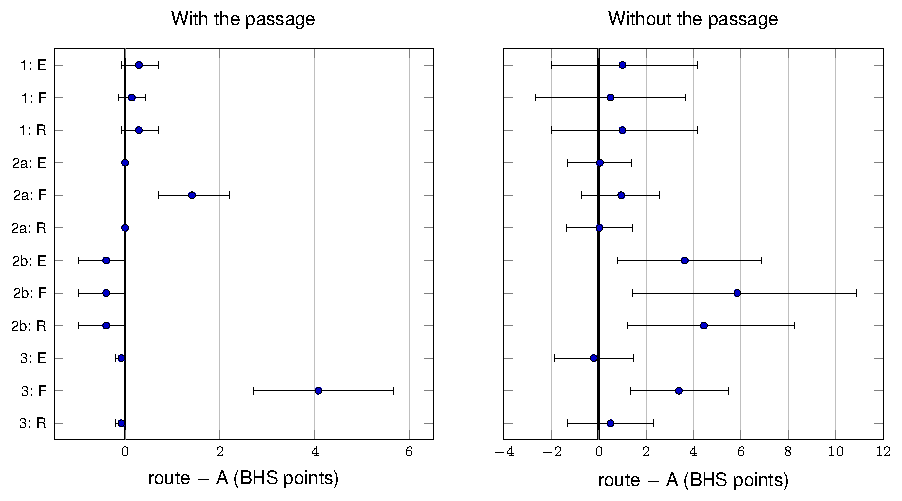
\includegraphics[width=\textwidth]{Fig1.pdf}
\caption{Route minus single best judge in all five tests (Study 1 is the registered test; 2a and 2b are splits;
3 is GenreHalluEval v2.0), with 95\% ranges. Points left of the thick line favour routing. No range lies wholly left
of 0; six lie wholly right of it.}\label{fig:forest}
\end{figure}

\begin{table}[t]
\centering\small
\caption{Study 3, GenreHalluEval v2.0 test half: errors and \BHS{} of each route. With the passage there are 300
correct and 1,200 hallucinated answers; without it the same numbers. Main tests: Holm over 6.}\label{tab:v2}
\begin{tabularx}{\textwidth}{@{}llrrrr>{\raggedright\arraybackslash}X@{}}
\toprule
Condition & Route & False alarms & Misses & \BHS{} & Holm $p$ & Judges used (answers) \\
\midrule
with passage & A & 0 & 7 & 0.29 & -- & gemma4 1,500 \\
 & E & 0 & 5 & 0.21 & 1.00 & gemma4 1,375; qwen3.5 125 \\
 & R & 0 & 5 & 0.21 & 1.00 & gemma4 1,360; qwen3.5 140 \\
 & F & 6 & 81 & 4.38 & $<$0.001 & gemma4 930; gpt-oss 210; tigerllm 170; qwen3.5 155; deepseek 35 \\
\midrule
without passage & A & 59 & 272 & 21.17 & -- & gemma4 1,500 \\
 & E & 53 & 291 & 20.96 & 1.00 & gemma4 760; qwen3.5 740 \\
 & R & 58 & 288 & 21.67 & 1.00 & gemma4 735; qwen3.5 695; gpt-oss 60; deepseek 10 \\
 & F & 70 & 309 & 24.54 & 0.006 & gemma4 625; qwen3.5 435; gpt-oss 245; tigerllm 145; deepseek 50 \\
\bottomrule
\end{tabularx}
\end{table}

%==================================================================================================================
\section{Analysis}
%==================================================================================================================

\subsection{Why routing has little room: one judge dominates}

On the v2.0 learn half, gemma4-31b is the best judge in 11 of 12 genres with the passage, and most genre cells are
decided by 0 to 2 errors. A route can only help where another judge is reliably better than the single best one, and
such genres hardly exist. Without the passage, qwen3.5-27b leads in six genres on the learn half, but only two of the
twelve best-versus-runner-up gaps are clear (both in genres where gemma4-31b leads), and no LLM is clearly better inside
the genre it named itself than inside the human genre.

\subsection{Learn-half leaders do not hold}

Where a different judge did lead on the learn set, the lead tended to shrink or reverse on new questions, as expected
when a winner is picked from many noisy cells. In Study 2b, qwen3.5-27b led in History and Religion on the learn half
and made more errors than A on those answers in the test half (21 vs 18 and 13 vs 5). In Study 3, qwen3.5-27b led
Education without the passage on the learn half (33.75 vs 35.75 for the runner-up); on the test half, E's Education
score was 31.0 against A's 23.5. Finer genres make each cell smaller and this effect stronger, not weaker.

\subsection{Why own-genre routing fails}\label{sec:whyf}

A judge needs an own-genre cell of 50 or more learn questions to be routed to. On the v2.0 learn half, gemma4-31b and
qwen3.5-27b named Geography, Culture and Religion for fewer than 50 questions each, so they had no cell there, while
weaker LLMs, which over-use some genres, did. F does not compare a cell with A, so it sends those questions to the only
LLM that has a cell: Geography mostly to tigerllm-9b (with the passage, 24.0 on that genre against A's 0.0) and
Culture to gpt-oss-20b. The better a strong judge names genres, the fewer genres it names often enough to own a cell.
R avoids this failure because it compares every own-genre path with the our-genre path, and it stays close to A.

\subsection{Small gains and their price}\label{sec:cost}

Routing was slightly ahead of A in some comparisons. We list every such case in Table~\ref{tab:smallgains}, with the
answers behind it and the cost of the route at test time.

\begin{table}[t]
\centering\small
\caption{Every case in which a route was ahead of A in the point estimate, and what it cost. Errors are counted on
the same test answers. Cost is for the whole test notebook of the route (both conditions) relative to A's notebook.
None of these differences is clear.}\label{tab:smallgains}
\begin{tabularx}{\textwidth}{@{}>{\raggedright\arraybackslash}p{2.6cm} >{\raggedright\arraybackslash}p{1.5cm} >{\raggedright\arraybackslash}p{1.3cm} >{\raggedright\arraybackslash}X >{\raggedright\arraybackslash}X@{}}
\toprule
Study, condition & Route & Gain & Answers behind the gain & Cost relative to A \\
\midrule
2b, with passage & R (= D, E, F) & 0.40 & 2 fewer misses (2 vs 4 of 252 hallucinations) & 1.9$\times$ calls, 4.2$\times$ prompt tokens, 3.0$\times$ wall time (all routes in one notebook) \\
3, with passage & E & 0.08 & 2 fewer misses (5 vs 7 of 1,200) & 1.2$\times$ calls, 2.7$\times$ tokens, 1.6$\times$ time \\
3, with passage & R & 0.08 & 2 fewer misses (5 vs 7) & 1.6$\times$ calls, 6.6$\times$ tokens, 2.5$\times$ time \\
3, without passage & E & 0.21 & 6 fewer false alarms but 19 more misses (344 vs 331 errors in all) & 1.2$\times$ calls, 2.7$\times$ tokens, 1.6$\times$ time \\
2a, 400 random splits, without passage & R, E & 0.09, 0.18 (mean) & better in 56\% and 55\% of the splits & not measured (saved runs) \\
\bottomrule
\end{tabularx}
\end{table}

Three observations make these gains unattractive.

\paragraph{The gains are as small as the judges' own noise.} The same judge, given the same prompt at temperature 0,
did not always return the same verdict in two notebooks: in Study 3, 3,258 of 3,270 shared (judge, answer) pairs agreed
(99.63\%), and gemma4-31b alone flipped 6 of 2,135 verdicts between the route-E and the single-best notebooks, four of
them in E's favour. The likely cause is batched GPU inference. A gain of two answers in 1,500 is of the same size.

\paragraph{A lower \BHS{} can hide more errors.} Without the passage, E's score is 0.21 lower than A's, but E makes
more errors in total (344 against 331): it removes 6 false alarms, which \BHS{} weights four times as much because
correct answers are rarer, and adds 19 misses. Whether this is a gain depends on what a user values.

\paragraph{The cost is several times higher.} Every route must first ask one or more LLMs for the genre, with a long
genre prompt, and must keep more than one judge available. In Study 3, against A's 3,000 calls, 0.55 million prompt
tokens and 1 h 22 min, E used 3,600 calls, 1.46 million prompt tokens and 2 h 10 min; R used 4,800 calls, 3.59 million
and 3 h 22 min; F used 6,000 calls, 5.74 million and 4 h 39 min. In the best case above (Study 3, E with the passage),
each answer that routing fixed cost about 300 extra calls and 0.45 million extra prompt tokens (counting the
whole notebook, both conditions). Learning the routes
cost more again: the v2.0 learn half took 33,000 calls and about 20 hours of model time, while choosing A needs only
the judge scores that any evaluation produces anyway.

\subsection{Genre guessing is not the bottleneck}

The genre guessers are accurate: on the v2.0 test half, gemma4-31b's genres agree with the human genres on 94.0\% of
questions and qwen3.5-27b's on 94.7\%. E and R therefore get the genre right almost always; they fail to help because
the best judge for the genre is usually the single best judge anyway.

%==================================================================================================================
\section{A noise- and cost-aware protocol for evaluating judge routing}\label{sec:protocol}
%==================================================================================================================

The analysis above suggests a general guardrail. Any change to a judge set-up (routing, a different judge, a different
prompt) should be accepted only if its gain is larger than the variation that the same set-up shows when it is simply
run again, and only if the gain is worth its cost. We propose five checks.

\begin{enumerate}
  \item \textbf{Measure the noise floor.} Run the reference judge on the same answers twice, or reuse every
  (judge, answer) pair that two runs share, and count the verdicts that differ. Let $\varphi$ be this flip rate and
  $N$ the number of test answers; about $\varphi N$ answers can change by chance alone.
  \item \textbf{Test on held-out questions.} Compare the new set-up with the reference on test items only, with a
  paired bootstrap over questions, and require the 95\% range to exclude zero.
  \item \textbf{Count the answers that changed.} Report the net number of answers fixed (errors of the reference
  minus errors of the new set-up), split into false alarms and misses. A gain smaller than about $\varphi N$ answers
  is indistinguishable from noise, and a lower \BHS{} with more errors in total is not a clear gain.
  \item \textbf{Price the gain.} Report the extra calls, prompt tokens and time, per answer fixed, including the
  one-off cost of learning the route.
  \item \textbf{Check coverage} (own-genre and other cell-based routes). For every genre, check which judge the route
  would use and compare its learn score with the reference; a cell-size rule must not hand whole genres to weak judges.
\end{enumerate}

Table~\ref{tab:protocol} applies the protocol to the cases where routing came closest to a gain.

\begin{table}[t]
\centering\small
\caption{The protocol applied. Flip rate: verdicts that differed when the same judge judged the same answer in two
notebooks. Net fixed: errors of A minus errors of the route on the same test answers (negative = the route made more
errors). Cost relative to A's notebook. No route passes.}\label{tab:protocol}
\begin{tabularx}{\textwidth}{@{}>{\raggedright\arraybackslash}p{2.4cm} >{\raggedright\arraybackslash}p{1.6cm}
>{\raggedright\arraybackslash}p{2.0cm} >{\raggedright\arraybackslash}p{2.3cm} >{\raggedright\arraybackslash}X
>{\raggedright\arraybackslash}p{1.8cm}@{}}
\toprule
Case & Flip rate & 95\% range excludes 0? & Net fixed & Cost (calls / prompt tokens) & Passes? \\
\midrule
Study 1, R, with passage & 3 / 920 (0.33\%) & no & $-4$ (9 vs 5 errors) & 1.8$\times$ / 5.1$\times$ & no \\
Study 2b, R, with passage & 1 / 425 (0.24\%) & no & +2 (2 vs 4 misses) & 1.9$\times$ / 4.2$\times$ & no \\
Study 3, E, with passage & 12 / 3,270 (0.37\%) & no & +2 (5 vs 7 misses) & 1.2$\times$ / 2.7$\times$ & no \\
Study 3, R, with passage & 12 / 3,270 (0.37\%) & no & +2 (5 vs 7 misses) & 1.6$\times$ / 6.6$\times$ & no \\
Study 3, E, without passage & 12 / 3,270 (0.37\%) & no & $-13$ (+6 false alarms fixed, $-19$ misses) & 1.2$\times$ / 2.7$\times$ & no \\
Study 3, F, with passage & 12 / 3,270 (0.37\%) & yes, worse & $-80$ (87 vs 7 errors) & 2.0$\times$ / 10.5$\times$ & no; fails coverage \\
\bottomrule
\end{tabularx}
\end{table}

With $\varphi \approx 0.3\%$ and $N=1{,}500$ answers per condition, about four to five answers can change by chance in
Study 3, more than the two answers that E and R fixed with the passage. The protocol is cheap: the noise floor comes
for free from any two runs that share a judge, and the other checks need only the saved outputs.

%==================================================================================================================
\section{Discussion}
%==================================================================================================================

\paragraph{What the result means.} Across five tests, with a change of dataset and without, with merged and with fine
balanced genres, and with cells of 20 and of 50 questions, routing hallucination judges by genre never beat the single
best judge. The simplest explanation is the one the data show directly: one strong judge (gemma4-31b, with qwen3.5-27b
close behind) is best or tied in almost every genre, and the differences between genres that remain are smaller than
the noise of picking winners from small cells. Genre routing can only pay off when judges have strong, stable and
different genre profiles. We did not find such profiles among current open-weight judges for Bangla QA.

\paragraph{Advice for practitioners.} Evaluate the candidate judges once, pick the best single judge, and report its
score with and without a reference. Treat any proposed improvement, routing included, with the protocol of
Section~\ref{sec:protocol}: if its gain is not larger than the judges' own run-to-run noise and not worth its cost,
keep the single best judge. GenreHalluEval v2.0 provides the split, labels and raw outputs to run these checks for new
judges without new data collection.

\paragraph{Limitations.}
\begin{itemize}
  \item \textbf{Written hallucinations.} All hallucinated answers were written by one LLM under a fixed guide, not
  produced by the judged models. Real hallucinations may be harder and may differ between genres.
  \item \textbf{Partly checked v2.0 data.} Claude wrote 970 of the 1,200 v2.0 questions; a 20\% sample was checked by
  two people, and the remaining labels are the design labels. Agreement with the design is an upper bound, because
  both annotators marked one correct answer per question.
  \item \textbf{Exploratory follow-ups.} Studies 2a, 2b and 3 were designed after the registered result. Study 3's
  tests were fixed in a dated file before its test runs, but not registered.
  \item \textbf{One run per setting.} Temperature 0 makes the runs nearly, but not fully, deterministic (99.6--99.7\%
  agreement across notebooks). All models are 4-bit quantised and served by one Ollama version.
  \item \textbf{Prompts and pool.} Instructions are in English for all judges except TigerLLM in Studies 2b and 3.
  The secondary pool with a commercial judge (GPT-4.1 mini) was not run.
  \item \textbf{Scope.} One language, one task (extractive QA with short answers) and genre as the only routing key.
  The passage-span shortcut (\BHS{} 13.8) shows that the with-passage condition is partly solvable without reading the
  question.
\end{itemize}

%==================================================================================================================
\section{Conclusion}
%==================================================================================================================

We release GenreHalluEval v2.0, a balanced 12-genre Bangla benchmark for hallucination judges with a fixed
learn/test split, double-checked labels and raw outputs of five judges, together with an audited BenHalluEval-QA set
and GenreHalluEval v1.1. On these sets, genre-aware routing did not make LLM hallucination judges better: in a
preregistered test and four follow-ups, no route was clearly better than the single best judge, and own-genre routing
was clearly worse in four of the eight study-and-condition pairs. The few small gains were within the judges' own
run-to-run noise while costing 1.2 to 1.9 times the calls and 2.7 to 6.6 times the prompt tokens. The noise- and
cost-aware protocol of Section~\ref{sec:protocol} turns this into a general check for judge set-ups. Future work should
test routing keys other than genre (for example answer type or difficulty), real model hallucinations, and settings in
which no single judge dominates.

\backmatter

%% Acknowledgements (optional): uncomment and fill in, e.g. the professor who reviewed the draft, if they agree.
%% \bmhead{Acknowledgements}
%% We thank ...

\section*{Statements and Declarations}

\bmhead{Funding}
No funding was received.

\bmhead{Competing interests}
The authors declare no competing interests.

\bmhead{Ethics approval and consent to participate}
Not applicable. No human participants took part other than
the authors, who labelled the data themselves; no personal data were collected.

\bmhead{Consent for publication}
Not applicable.

\bmhead{Data availability}
\url{https://github.com/Enigmah-00/GenreHalluEval}. The release contains the
three test sets, all labels and every raw model output. BenHalluEval-derived data are
released under its licence, CC BY-NC-SA 4.0; Wikipedia passages are CC BY-SA; the grammar-book and news passages
are used for research purposes under Bangladesh's Copyright Act 2023.

\bmhead{Code availability}
The analysis code, prompts and Kaggle notebooks are in the same repository
(\url{https://github.com/Enigmah-00/GenreHalluEval}), under the MIT License.

\bmhead{Preregistration}
Study 1 was registered on OSF before any test answer was judged
(\url{https://osf.io/fmbs8}; embargoed until 27 October 2027). Deviations are listed in the
registration's deviation log.

\bmhead{Use of large language models}
The use of a large language model (Claude, Anthropic) to write hallucinated
answers, part of the questions, draft genre labels and code, and help draft the text is documented in
Section~\ref{sec:llmuse}. The authors take full responsibility for the content.

\bmhead{ORCID iDs}
Mahdi Hasan Qurishi: \url{https://orcid.org/0009-0000-8112-167X};
Umme Zoayria Abedin: \url{https://orcid.org/0009-0002-4839-5120};
Md Saminul Amin: \url{https://orcid.org/0009-0007-4348-5094}.

\bmhead{Author contributions}
Mahdi Hasan Qurishi: conceptualisation, study
design, BenHalluEval genre verification and annotation (annotator 1), GenreHalluEval gold answers (genre annotator 3),
runs, writing. Umme Zoayria Abedin: GenreHalluEval answer labels (annotator 1 for v1.1 and the v2.0 check),
genre annotation, review. Md Saminul Amin: blind genre and answer labels for BenHalluEval (annotator 2), GenreHalluEval
answer labels (annotator 2 for v1.1 and the v2.0 check), genre annotation, review.

\begin{appendices}

\section{Hallucination writing and AI-written data}\label{app:ai}

Each hallucinated answer was written to be wrong by the passage, with no hedges, different from the other three
answers of its question, and of a fixed type: F (a wrong fact of the same kind as the gold), C (a misread question,
usually another span of the passage), S (the gold plus a false detail) and I (a wrong inference). An automatic check
rejected answers that equalled the gold or another answer. For Bangla grammar questions, wrong word splits avoided
spelling variants of the gold split, so that no hallucination could be read as a spelling difference. For GenreHalluEval
v2.0, the 20\% blind check of Section~\ref{sec:data} found every sampled question clear and answerable. Annotator 1
agreed with the design on all 970 answers; annotator 2 differed on 3 of 969 (one of them a question about a person's
birth name), and in all three the passage supports the design label. One further answer was edited by annotator 2
and is left out of the agreement.

\section{Settings of each study}\label{app:settings}

\begin{table}[h]
\centering\small
\caption{Learn and test sets, pools and locks.}
\begin{tabularx}{\textwidth}{@{}l X X r X@{}}
\toprule
Study & Learn & Test & Min.\ cell & A (with / without passage) \\
\midrule
1 & BenHalluEval-QA v1.3, 920 q., 9 judges & GenreHalluEval v1.1, 175 + 75 q. & 50 & gemma4-31b / gemma4-31b \\
2a & half of BenHalluEval, 459 q. & other half, 461 q. & 50 (also 25) & gemma4-31b / gemma4-31b \\
2b & GenreHalluEval v1.1, 125 q., 5 judges & 63 + 62 q. & 20 & qwen3.5-27b / gemma4-31b \\
3 & GenreHalluEval v2.0, 600 q., 5 judges & 300 + 300 q. & 50 & gemma4-31b / gemma4-31b \\
\bottomrule
\end{tabularx}
\end{table}

\end{appendices}

\bibliography{references}

\end{document}
